\section{The validation program}\label{sec:validation}

\evfut{} Nothing in this section has run; rules not yet registered are marked \enquote{proposed}.
The program asks for no money before its
cheapest decisive test has run, and each tranche is released only by a gate that reads CONTINUE. The
studies test one link at a time, and a failed link stops or reroutes everything above it: trustworthy
inputs (L0, V0), an informative absence check (L1, V1), retrospective prediction on published gold (L2,
V2), a measurable residual (L3, V4), prospective prediction (L4, V5, which decides H2) and practical
value (L5, V6--V8; V6 tests H3). \evint{} L1 comes first: with an uninformative closure step, a gold test
measures \enquote{a lens fired} plus density. The departure study V3 is off this chain; it tests H-OSS.

\begin{evfutbox}[float=tbp]
  \textbf{Gate rules, proposed for pre-registration.}\\[2pt]
  \textbf{MS1, closure verdict (end of Phase~0).} CONTINUE if human--human $\kappa \geq 0.70$ on the
  gating split (closed versus not closed), corpus-level retrieval recall meets its floor (proposed
  0.80), and at least one judge beats the fair control: its own-minus-control difference in the
  not-closed rate has a 95\% lower bound above 0 and lies within $\pm 0.10$ of the humans'. Otherwise STOP
  the automated absence check.\\[2pt]
  \textbf{MS3, screening gate for Phase~2 money (end of Phase~1).} CONTINUE only if the pooled
  retrospective $\Delta$AUROC has a point estimate $\geq \delta$, \emph{and} its lower 90\% bound is
  $> -\delta/2$, \emph{and} the map adds value over density and area size (conditional AUROC within
  density tertiles $\geq 0.5 + \delta$). Otherwise STOP H2 funding. MS3 is not a verdict on H2 and has no
  inconclusive route.\\[2pt]
  \textbf{MS5, H2 verdict (Phase~2).} STOP if the upper 90\% bound of the prospective $\Delta$AUROC is
  below $\delta$. CONTINUE if the lower 90\% bound is above 0 and the point estimate is at least
  $\delta$. Any other reading is reported as not supporting H2 and ends H2 funding.
\end{evfutbox}

\paragraph{Who reads the gates.} An external gate reader, an independent statistician or an advisory
board with one, reads MS1, MS3 and MS5 against the hash-committed pre-registration, with authority over
them. The reader is not a co-applicant and is not paid from a tranche the reading releases. Any owner
exception, at any gate, needs the reader's written sign-off, or the reading is void. \evobs{} No such
reader existed during the PoC, and none is named yet.

\subsection{Rules common to every study}

\evfut{} \emph{Two-step freeze.} The judge is chosen at MS1. Then MS2 (about month~4 of Phase~1)
hash-commits the pre-registrations, lexicons, thresholds, the adopted judge, the area score and the list
of eligible golds \parencite{nosek2018preregistration}. Only then is gold acquired and are held-out
domains reconstructed. \emph{Area score.} Every decisive test ranks areas, so Phase~1 builds a fixed
aggregation (for example the maximum or a noisy-OR) over the \emph{uncapped} candidates in each area,
chosen on pilot data only. \emph{Density.} Candidacy and rank are built from source counts, so a plain
gain over density is close to testing a variable against itself. The primary incremental analysis is the
area score's AUROC within density tertiles. \emph{Domains and dated corpora.} PLC and GDPR serve only for
debugging, V1 and an unanalyzed V5 pilot. Decisive studies use held-out domains on a corpus dated before
the criterion (archive captures and publications dated before the cutoff), with a per-gold blocklist and
a memorization probe on every model in the chain \parencite{golchin2023time,sainz2023nlp}.
\emph{Judges.} No LLM judge is a criterion. One is adopted only from another family than the generator,
with $\kappa \geq 0.70$ against blind human coders (the adoption rule), and re-checked on each new text
type before gold is unsealed; where it fails, closure there is human-coded.

\evfut{} \emph{Statistics.} Area-level AUROC is compared by DeLong's method or a cluster bootstrap
\parencite{delong1988comparing,obuchowski1997nonparametric}, with the strongest baseline chosen inside
each resample; MS5 has the logic of two one-sided tests \parencite{lakens2017equivalence}.
\emph{Choosing $\delta$.} Proposed $\delta = 0.05$: a smaller gain over density is unlikely to justify
reconstruction, while 0.10 would let a stop rule kill a real, modest gain. Under planning assumptions
without empirical basis (Hanley--McNeil errors, AUROC 0.70 against 0.62, error correlation 0.5;
\cite{hanley1982meaning}), the 90\% half-width of $\Delta$AUROC is about $\pm 0.14$ with 20 areas per
class, $\pm 0.10$ with 40, $\pm 0.06$ with 100 and $\pm 0.05$ with about 150.

\begin{figure}[tbp]
  \centering
  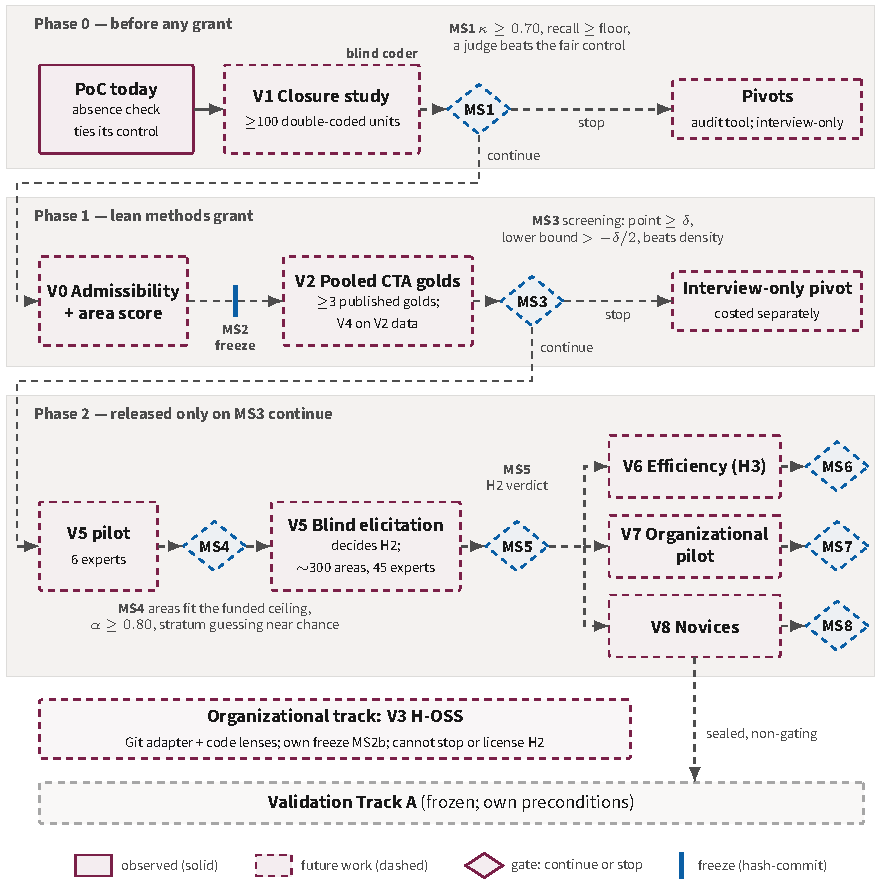
\includegraphics{figures/pdf/fig13_validation.pdf}
  \caption[The validation program]{Which studies, in which order, turn gap candidates into validated
    predictions, and which gate releases which money? Phase~0 (V1) ends at MS1. Phase~1 (V0, the MS2
    freeze, pooled V2, V4) ends at the MS3 screening gate. In Phase~2, V5 decides H2 at MS5 after its
    pilot gate MS4; only then do V6 (H3), V7 and V8 follow. V3 tests the separate hypothesis H-OSS.
    Stops lead to pivots. Track~A runs on a separate rail. All elements except the PoC are future work.}
  \label{fig:validation}
\end{figure}

\subsection{The studies}

Each study below is given by its design, people, measure, sample size and gate; the full protocols
and a per-study table are in the Extended Technical Report, Section~17.

\paragraph{Phase~0 --- V1, the closure study (before any grant).} \evfut{} \emph{Units:} a lens
firing with its seed span, missing element and evidence pool, in both arms of the fair control. All 107
admissible firings (PLC 56, GDPR v1 51) in both arms give 214 units; about 100 units from one new
non-gold domain are added so that no judge is scored only in-sample. \emph{Coders:} the judgment is
textual, so coders need codebook training, not domain expertise. The non-owner coder and the owner
(under origin blinding) code every unit, blind to arm, judge answer, rank and run. \emph{Retrieval
recall:} for about 50 firings the coder searches the ledger's full snapshots for the missing element.
\emph{Judges:} the local 7B model, a stronger open-weight model, and frontier models from other
families. \emph{Sample size:} with balanced classes, $\kappa \approx 0.70$ has a 95\% half-width of about
$\pm 0.10$ at 214 units. \emph{Cost:} tens of coder hours plus local compute, on the order of
EUR~$10^3$. \emph{On STOP:} pivot to reconstruction as a documentation-audit tool, or to interviewing
without a gap map.

\paragraph{Phase~1 --- V0, V2 and V4.} \evfut{} \emph{V0} makes pipeline outputs admissible as code,
builds the dated-corpus mode and the area score, and runs N2's deferred protocols after a calibration
pilot; its gate is the MS2 freeze (no hash, no gold). \emph{V2} scores the frozen gap map against
several published CTA task lists, pooled. A gold is eligible if it is an itemized list of steps,
decisions or cues from more than one expert, in a domain other than PLC, GDPR or Track~A physics, with
a dated corpus above a floor. Named candidates, in order: Sullivan's cricothyrotomy list, the only one
confirmed as itemized \parencite{sullivan2014use}; the NICU cue study \parencite{crandall1993critical};
the troubleshooting study \parencite{chao1994percentage}; and the PARI guide
\parencite{hall1995procedural}. Proposed: at least three golds, four to six if eligible. Each gold
domain is reconstructed once, from its dated corpus, before the sealed gold is acquired. Baselines
include random, area size, retrieval density, corpus frequency, a type prior from the other golds and a
plain-LLM ranking. \emph{What MS3 can read:} at four golds and 80 areas split evenly, the half-width is
about $\pm 0.10$, so CONTINUE needs a point estimate of at least 0.075. A map with no true gain passes
with probability about 0.11; a true gain of $\delta$ passes with about 0.34. \evint{} MS3 is a screen: it
accepts about a one-in-nine chance of releasing Phase~2 for a useless map, which V5 then stops. \emph{V4}
checks unseen-item estimators on V2 data against known truth; out of tolerance, only observed counts are
reported. It does not gate.

\paragraph{Phase~2 --- V5, blind prospective elicitation, which decides H2.} \evfut{} \emph{Design:}
freeze reconstruction, dated corpus, gap map, area score and partition. Sample areas in four labeled
strata: top of the area score (G), lowest retrieval density (D), top of a plain-LLM ranking (L) and
random (R). Each area gets a neutral CDM-style probe of about 8 minutes, the same for every area and
never the gap map's own question \parencite{klein1989critical}. \emph{Domains and people:} a PLC pilot,
not analyzed for effect; the main study in two held-out domains. Practitioners with several years of
practice, outside any Track~A pool, three per area \parencite{chao1994percentage}; one interviewer per
domain, two blind coders. \emph{Outcome:} an item counts if it is absent from the frozen reconstruction
\emph{and} the dated corpus, and is corroborated by a second expert, a trace or an outside artifact;
importance is rated blind to stratum. \emph{Blinding:} experts are told the study maps where practice
relies on unwritten knowledge, not that a model chose areas (partial disclosure, stated in the ethics
application, with debriefing). Interviewers see only area names in random order; a guess-the-stratum
check on 20\% of areas reports leakage. \emph{Sample size:} about 150 residual-present and 150 other
areas (300), 900 probes, about 45 experts at 20 areas each plus 6 in the pilot: about 150--250 expert
hours and 1,200--1,900 coder hours, roughly EUR~40--160k before staff time. \emph{Gates:} \textbf{MS4}
releases the main study only if the pilot (6 experts $\times$ 20 areas, 40 areas) projects at most 450
areas, segmentation reaches $\alpha \geq 0.80$, and stratum guessing stays near chance; otherwise V5 stops
and H2 is reported as untested prospectively. No underpowered V5 is ever run. \textbf{MS5} then reads its rule
in the gate box.

\paragraph{Phase~2 --- V6, V7, V8, only on MS5 CONTINUE.} \evfut{} \emph{V6 (H3, gate MS6)} is a
within-expert crossover of targeted questions against a standard unprompted-then-CDM interview; the
breadth ranking and selection by expected information gain (not built) are separate arms
\parencite{lindley1956measure}. Items first seeded by a question count only if independently
corroborated \parencite{loftus1975leading}. CONTINUE if the lower 90\% bound of the items-per-hour ratio
exceeds 1 and the point estimate is at least 1.25; STOP if the upper bound is below 1.25; any other reading
counts against H3. \emph{V7 (gate MS7)} is a descriptive pilot in one partner organization with 6--12
staff experts, after the deferred N2 validation; it goes multi-partner only if G areas beat D and R in
both parts. \emph{V8} covers the learner side: public learner data (no gate), 30--60 novices on confirmed
residual areas (MS8), and Track~A, touched only through sealed, secondary, non-gating predictions.

\paragraph{Organizational track --- V3 (H-OSS).} \evfut{} None of its components exists: a Git adapter
that turns commits, issues and reviews into claims with exact spans, areas mapped to code units at a
time before a departure, and lenses for code text, frozen at MS2b once the adapter exists. The outcome is
blind-coded rationale-seeking issues and defect-fix commits after truck-factor departures
\parencite{avelino2016novel}, analyzed as a staggered difference-in-differences
\parencite{callaway2021difference}, against baselines that include authorship concentration and knowledge
at risk \parencite{rigby2016quantifying}. A 5-departure pilot sizes the study; its gate uses the MS5 rule
on H-OSS only. It can neither stop nor license H2.


\evint{} Each STOP teaches something. At MS1 it shows that absence in text cannot yet be judged
reliably, and it leaves a public closure set. At MS3 it leaves a reconstruct-versus-CTA benchmark. At
MS5 it falsifies, with a bounded effect size, the claim that text reconstruction locates the human
residual. Program threats (incomplete gold, method-dependent elicitation, matcher error) are treated
there too.
